% Build: latexmk -pdf -use-biber main.tex
% v2 (2026-08-19): rewritten to the settled Stage-5 skeleton (5단계_논문_골격.md v0.1):
% honest measurement study + automation + quantified negative result. Data: 논문_데이터_표.md.
\documentclass[11pt,a4paper]{article}
\usepackage[margin=1in]{geometry}
\usepackage{microtype,amsmath,amssymb,booktabs,xcolor,enumitem,hyperref}
\usepackage{tikz}
\usetikzlibrary{positioning,calc,patterns,arrows.meta,decorations.pathreplacing}
\usepackage[nameinlink,noabbrev]{cleveref}
\usepackage[backend=biber,style=alphabetic,maxbibnames=99]{biblatex}
\addbibresource{../references.bib}
\hypersetup{colorlinks=true,allcolors=blue}
\newcommand{\todo}[1]{\textcolor{red}{[TODO: #1]}}
\newcommand{\xwing}{X-Wing}\newcommand{\slothy}{SLOTHY}\newcommand{\keccak}{Keccak-f1600}
\title{Stitching Hybrid Key Exchange on an In-Order Dual-Issue Cortex-M85:\\
An Honest Measurement Study with Automated Two-Stream Scheduling}
\author{Anonymous Author(s)}\date{}
\begin{document}\maketitle

\begin{abstract}
Function stitching---interleaving two independent cryptographic computations into one
instruction stream---was proposed by Intel for out-of-order x86 cores. We ask what
happens when the idea is carried to a post-quantum/traditional hybrid KEM
(X25519 $\times$ the Keccak component of ML-KEM) on an in-order dual-issue embedded
core (Cortex-M85). We (i) build an automated pipeline that extends the \slothy{}
superoptimizer to two-stream scheduling under carry-flag and register-file
constraints; (ii) measure, on silicon, both the pre-registered upper bound of the
technique (21--27\% per \xwing{} operation) and the recovery actually achieved
(7--11\%), and decompose the gap into its causes by isolating experiments; and
(iii) obtain, as an independent by-product, a 4-way MVE-batched \keccak{} that is
18\% faster per state than the pqm4 scalar baseline. Our conclusion is honest:
on an in-order core, instruction-level stitching of this pair is a real but thin
net win, and the thinness is not an accident of tuning but structural---register
pressure converts to a fixed yield tax, spill traffic contends for the load/store
unit, and store issue blocks scalar co-issue entirely. All claims are backed by
cycle-exact measurements on an EK-RA8M1 board with pre-registered decision gates,
and the toolchain, harness, and all kernels are published as artifacts.
\end{abstract}

\paragraph{Keywords.} PQ/T hybrid; \xwing{}; ML-KEM; X25519; \keccak{}; function
stitching; superoptimization; \slothy{}; Cortex-M85; MVE.

\section{Introduction}\label{sec:intro}

The transition answer to quantum-capable adversaries is hybrid key establishment:
\xwing{} \cite{XWing24} runs X25519 and ML-KEM-768 and combines their secrets, so
that either assumption alone suffices. The price is that both algorithms execute.
On desktop-class cores this hybrid tax is noise; on the microcontrollers that
anchor embedded TLS stacks it is a deployment argument. Existing mitigations make
each primitive faster in isolation, or spend more silicon---a second core
\cite{DualCore25,ParHyb26}. This paper evaluates a third option on a single core:
\emph{hide one algorithm in the issue slots the other wastes}.

The opportunity is microarchitectural. Cortex-M85 is an in-order, dual-issue
Armv8.1-M core. X25519 field arithmetic is a long dependency chain of
\texttt{umaal} multiply-accumulates and \texttt{adds}/\texttt{adcs} carries: we
measure IPC 1.03, i.e.\ 48.7\% of the two-issue capacity idles
(\cref{sec:bounds}). The \keccak{} permutation that dominates ML-KEM's symmetric
cost is dense, independent bitwise work (IPC 1.66), and it exercises the
ALU/shift resources rather than the multiplier. The two computations are
complementary in exactly the sense Intel's function-stitching white paper
\cite{Intel10} exploited for AES$\times$SHA-1---but that work targeted
out-of-order x86, placed instructions by hand at source level, never measured the
idle capacity it claimed to fill, and paired only symmetric primitives.

We transplant the idea and, deliberately, test it to destruction. Concretely:

\begin{enumerate}[leftmargin=*]
\item \textbf{Automation: a two-stream extension of \slothy{}}
      (\cref{sec:auto}). We extend the constraint-solving superoptimizer
      \cite{Slothy22} with the missing scalar instruction classes, APSR
      (carry-flag) lifetimes as solver dependencies, a scalar dual-issue
      execution model, and a MAC-accumulator forwarding rule---validated on
      silicon at 17, 156, and 1,184-instruction scale. Fed nothing but the
      concatenation of two independent streams, the solver discovers the
      interleaving and reallocates registers \emph{across} streams, beating the
      best manual stitch at every scale and beating a strong serial baseline
      built from hand-optimized parts.
\item \textbf{A quantified account of why recovery is thin}
      (\cref{sec:causes}). The pre-registered per-operation bound is 21--27\%;
      the end-to-end recovery is 7--11\%. We attribute the gap cause by cause
      with isolating experiments: spill self-cannibalization (a full-ratio
      kernel yields 3.3\%), a structural register-yield tax (+12--14\%
      regardless of how few registers are ceded), LSU contention (58\% hiding
      for a pure MAC chain vs.\ 27\% with spill traffic), and multiplier
      monopoly (scalar$\times$scalar NTT-style pairing hides $-1$\%). A pairing
      spectrum experiment pins the co-issue ceiling to one instruction class:
      \texttt{vstrw} blocks scalar issue for both of its cycles, and a
      three-term model then reproduces the measured stitched time with zero
      error.
\item \textbf{A 4-way MVE-batched \keccak{}} (\cref{sec:planb}): four
      permutation states in vector registers, 188.5 cycles per state and round
      vs.\ 229 for the pqm4 scalar baseline ($-18$\%), using zero scalar data registers.
      This is an independently useful result for any Armv8.1-M ML-KEM.
\item \textbf{Pre-registered methodology} (\cref{sec:bounds}). Every
      go/no-go in this project was written down before measuring: a kill gate
      after the bound measurement, a 20\% bar for the end-to-end phase, and a
      declared fallback narrative. We report against those commitments,
      including the parts that failed them.
\end{enumerate}

The paper's shape is unusual on purpose: the strongest deliverables are a tool,
a decomposition of a negative-leaning result, and a by-product kernel. We think
this is what an honest evaluation of a plausible idea should look like.

\section{Background}\label{sec:background}

\subsection{Function stitching and its promise}
Intel's white paper \cite{Intel10} interleaves two independent computations so
that stalls of one are filled by the other, with the ideal
$T_{\text{stitch}} \approx \max(T_A, T_B)$: the shorter computation becomes
free. The report is source-level and hand-scheduled, gives no measurement of the
idle capacity being filled, and relies on out-of-order hardware to absorb
scheduling imperfections. One principle we adopt directly: gains must be
reported against the \emph{strongest} serial baseline available, including
optimizations of the baseline itself found during the work.

\subsection{Cortex-M85: the arithmetic of the ceiling}
An in-order dual-issue core bounds slot recovery at 50\% (Intel's 4-issue
Westmere wasted up to 75\%). No hardware reordering exists, so a static
schedule's quality \emph{is} its performance---which cuts both ways: stitching
must be scheduled perfectly to work, and a constraint solver, not hand
placement, is the natural tool. We pin code in ITCM and data in DTCM (both
0-wait) to remove memory-hierarchy variation.

\subsection{\xwing{} and its Keccak share}
\xwing{} \cite{XWing24} = X25519 + ML-KEM-768 + a SHA3-256 combiner. Key
generation runs one X25519 scalar multiplication, encapsulation two,
decapsulation one; the ML-KEM sides invoke \keccak{} 43, 44, and 44 times
respectively (measured), plus one combiner permutation. The natural stream pair
is therefore X25519 (MAC-bound stream A) $\times$ Keccak (ALU-bound stream B).

\subsection{\slothy{}}
\slothy{} \cite{Slothy22,SlothyM7_25} solves instruction scheduling and register
allocation jointly with CP-SAT, for a \emph{single} input stream. Its
Armv8.1-M model is MVE-centric: the scalar classes X25519 needs
(\texttt{umull}/\texttt{umaal}, carry arithmetic) were absent, scalar dual issue
was not modeled (issue rate 1), and flag lifetimes were not constraints. Those
are precisely the extensions of \cref{sec:auto}.

\section{Pre-Registered Bounds: How Much Is There to Win?}\label{sec:bounds}

\paragraph{Method.} All measurements: EK-RA8M1 (Cortex-M85, 480\,MHz), GCC
13.2.1 \texttt{-O2}, code in ITCM, data/stack in DTCM, DWT \texttt{CYCCNT},
$N{=}100$ medians, 25-cycle harness calibration subtracted. Instruction counts
come from Unicorn emulation, cross-checked on two unrelated inputs (equal counts
double as a constant-time check, \cref{sec:ct}). Emulation is used only for the
\emph{numerator}: both kernels are secret-independent straight-line code, so the
instruction count is a deterministic constant rather than an estimate, and every
cycle figure is measured on silicon. The residual uncertainty is definitional---the
emulator charges IT-block bodies individually, which can differ from
\texttt{INST\_RETIRED} by a few percent---so slot-waste figures carry roughly
$\pm1$ percentage point. Functional gates: RFC~7748
KATs \cite{RFC7748}, SHA3-256 KATs, ML-KEM-768 round trip \cite{FIPS203} on
pqm4 \cite{pqm4} and a Lenngren X25519 \cite{Lenngren}---all pass on the board.
Before measuring we registered the decision rule: bound ${<}15\%$ kills the
project, $15\%\leq b<30\%$ forces a reduced two-week pilot, ${\geq}30\%$ proceeds.

\begin{table}[t]\centering
\caption{Stand-alone measurements and slot waste (median cycles).}
\label{tab:base}
\begin{tabular}{lrrrr}\toprule
Kernel & Cycles & Instructions & IPC & Slot waste\\\midrule
X25519 scalar mult (Lenngren) & 357,474 & 366,934 & 1.03 & \textbf{48.7\%}\\
\keccak{} (pqm4) & 5,526 & 9,162 & 1.66 & 17.1\%\\
ML-KEM-768 keygen/encaps/decaps & 437k/453k/504k & \multicolumn{3}{c}{(43/44/44 permutations)}\\
SHA3-256 combiner (134\,B) & 7,648 & --- & --- & ---\\\bottomrule
\end{tabular}\end{table}

\Cref{tab:base} quantifies what Intel never measured: the idle capacity.
X25519's dependency chains leave $2{\cdot}357{,}474-366{,}934 = 348{,}014$
empty issue slots per scalar multiplication. Charging Keccak's instructions
against those slots (and capping by stream length) yields \cref{tab:bound}:
21--27\% per \xwing{} operation, average 23.9\%. The slot term assumes every
idle slot is fillable by the partner stream---optimistic on an in-order core,
but \cref{sec:auto} measures IPC 1.99 on a 1:1 interleave, within 0.5\% of the
two-issue floor, which retrospectively justifies it. Two structural observations:
(i) encapsulation is limited by stream length---two scalar multiplications
provide more idle slots than Keccak has instructions; (ii) on M85 the Keccak
stream is the \emph{shorter} one, so coverage dilution---not slot capacity---sets
the bound. This is what our pre-registration anticipated: the plan predicted from
M4 accounting \cite{Sim26} that X25519 would be the longer stream and that
coverage would dilute, and the M85 measurement confirms that direction. The
gate verdict, mechanically applied: $23.9\% \in [15\%,30\%) \Rightarrow$
pilot.

\begin{table}[t]\centering
\caption{Pre-registered overlap upper bounds per \xwing{} operation.}
\label{tab:bound}
\begin{tabular}{lrr}\toprule
Operation & Overlappable cycles & Bound\\\midrule
Key generation & 209,905 & 26.4\%\\
Encapsulation & 248,670 & 21.2\%\\
Decapsulation & 209,905 & 24.2\%\\\bottomrule
\end{tabular}\end{table}

\begin{figure}[t]\centering
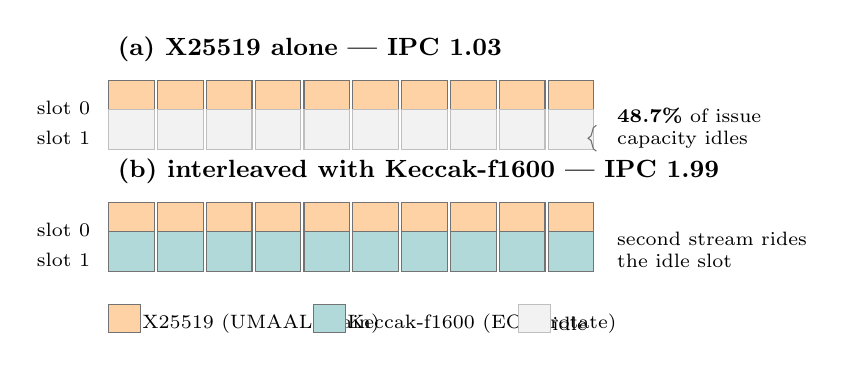
\begin{tikzpicture}[x=0.62cm,y=0.62cm,font=\scriptsize]
  \tikzset{
    slot/.style={draw=black!55,minimum width=0.58cm,minimum height=0.5cm,
                 inner sep=0pt,anchor=south west},
    used/.style={slot,fill=orange!35},
    idle/.style={slot,fill=black!5,draw=black!25},
    keca/.style={slot,fill=teal!30},
  }
  % ---- (a) X25519 alone ----
  \node[anchor=south west,font=\small\bfseries] at (0,3.05) {(a) X25519 alone --- IPC 1.03};
  \node[left=3pt,anchor=east] at (0,2.3) {slot 0};
  \node[left=3pt,anchor=east] at (0,1.7) {slot 1};
  \foreach \i in {0,...,9} {
    \node[used] at (\i,2.05) {};
    \node[idle] at (\i,1.45) {};
  }
  \node[right=4pt,anchor=west,align=left] at (10,1.9)
       {\textbf{48.7\%} of issue\\capacity idles};
  \draw[decorate,decoration={brace,amplitude=3pt},black!55]
       (10,1.42) -- (10,1.95);
  % ---- (b) interleaved ----
  \node[anchor=south west,font=\small\bfseries] at (0,0.55) {(b) interleaved with \keccak{} --- IPC 1.99};
  \node[left=3pt,anchor=east] at (0,-0.2) {slot 0};
  \node[left=3pt,anchor=east] at (0,-0.8) {slot 1};
  \foreach \i in {0,...,9} {
    \node[used] at (\i,-0.45) {};
    \node[keca] at (\i,-1.05) {};
  }
  \node[right=4pt,anchor=west,align=left] at (10,-0.6)
       {second stream rides\\the idle slot};
  % ---- legend ----
  \node[used,minimum width=0.4cm,minimum height=0.35cm] at (0,-2.3) {};
  \node[anchor=west] at (0.5,-2.12) {X25519 (UMAAL chain)};
  \node[keca,minimum width=0.4cm,minimum height=0.35cm] at (4.2,-2.3) {};
  \node[anchor=west] at (4.7,-2.12) {\keccak{} (EOR/rotate)};
  \node[idle,minimum width=0.4cm,minimum height=0.35cm] at (8.4,-2.3) {};
  \node[anchor=west] at (8.9,-2.12) {idle};
\end{tikzpicture}
\caption{Why stitching should pay on an in-order dual-issue core. The
multiply-accumulate chain of a Montgomery ladder step serialises on its own
carry dependencies, leaving one of the two issue slots empty in 48.7\% of
cycles (measured, \cref{tab:base}). A second, register-disjoint instruction
stream can occupy that slot without displacing the first---the microbenchmark
of \cref{sec:auto} reaches IPC 1.99, the two-issue floor. The gap between this
picture and the 7--11\% actually recovered is the subject of this paper.}
\label{fig:slots}
\end{figure}

\section{Automation: Two-Stream \slothy{}}\label{sec:auto}

\subsection{Feasibility by hand first}
Microbenchmarks establish that the hardware digests interleaving: a 1:1 mix of a
UMAAL chain with a non-flag-setting \texttt{eor}/rotate chain runs at IPC 1.99
(within 0.5\% of the two-issue floor), hiding 80\% of the shorter stream.
Making the second stream memory-resident changes the saving by 2 cycles in
4,000: LSU traffic pairs with the MAC stream, so \emph{the stitching-specific
spill penalty is zero}. Reserving 4 (even 8) registers for stream B costs a
compiled stream A nothing measurable---but that holds only where the compiler
still has spill headroom; the hand-tuned fiat multiply pays a 12--14\% yield tax
instead, which is why the microbenchmark result must not be read as a general
one (quantified below). A scripted ``zipper'' stitcher then
produces KAT-validated real kernels; its best manual result, 681 cycles for a
256-bit multiply plus a full Keccak round, is still $1.09\times$ a
626-cycle strongest-serial baseline---and manual sweeps plateaued there. That
gap is a register-allocation-plus-scheduling co-optimization problem: the
solver's job description.

\subsection{What the solver needed}
Our patch (published; upstream model at \texttt{241093fa5ddc}) contributes,
in order of discovery, each item forced by a measured failure:
\begin{itemize}[leftmargin=*]
\item \textbf{19 scalar instruction classes} absent from the Armv8.1-M model
      (\texttt{umull}, \texttt{umaal}, carry arithmetic incl.\ immediate forms,
      \texttt{umlal}, shifted/flag variants, \ldots).
\item \textbf{APSR lifetimes as dependencies}
      (\texttt{modifiesFlags}/\texttt{dependsOnFlags}): X25519 carry chains
      survive any legal schedule by construction, mechanizing the one hazard
      that Intel's symmetric-only pairing let them ignore.
\item \textbf{Scalar dual issue}: issue rate $1\to2$ plus a second scalar ALU
      slot (MAC and LSU unchanged).
\item \textbf{MAC accumulator forwarding} (model v0.3): silicon executes a
      dependent \texttt{umaal} chain at 1 cycle/instruction through the
      accumulator operand; the stock 2-cycle latency mis-priced stream A by
      $2\times$ and made the solver \emph{lose} to the zipper (1,319 vs.\
      1,018 cycles) until fixed---after which it wins (996). Model accuracy is
      not a nicety; on an in-order core it decides the outcome.
\item \textbf{Three safe-transform rules} for feeding compiler output to the
      solver, each validated by a corruption we debugged to zero: split
      doubleword accesses (the model treats \texttt{ldrd}/\texttt{strd} as
      4-byte), never reuse a spill slot (WAR/WAW memory anti-dependencies are
      not preserved), and order base-destroying load pairs last. Reported
      upstream as three issues.
\end{itemize}
Input needs no annotation: the two streams are concatenated (or pre-zipped, see
below) and dependency analysis discovers their independence.

\subsection{Validation ladder}
\begin{table}[t]\centering
\caption{Serial vs.\ best manual stitch vs.\ solver, board-measured
(cycles/iteration, correctness-checked against C references).}
\label{tab:solver}
\begin{tabular}{lrrrr}\toprule
Scale & Serial & Manual & \slothy{} & Solver vs.\ manual\\\midrule
17 instr (concept) & 13.06 & --- & 11.07 & ($-15\%$ vs.\ serial)\\
156 instr & 110.06 & 88.07 & 85.06 & $-3.4\%$\\
1,184 instr (full kernel) & 727.0 & 681 & 657.0 & $-3.5\%$\\
1,130 instr (fiat carry-mul) & 702.0 & --- & 630.0 & ($-10.3\%$ vs.\ serial)\\
1,110 instr (bit-interleaved) & 636.0 & --- & \textbf{579.0} & ($-9.0\%$ vs.\ serial)\\
Co-issue 1,222 instr (scalar$\times$MVE) & 1,365 & 1,018 & \textbf{996} & $-2.2\%$\\\bottomrule
\end{tabular}\end{table}

\Cref{tab:solver} is the tool's report card. Three points. First, the solver
beats the best manual stitch wherever one exists, and at full scale the manual
technique \emph{cannot even be constructed}: the zipper's premise---a static
register partition between streams---collapses when stream A uses all
registers freely (we demonstrated the resulting live-value corruption as a
hard fault); the solver, allocating globally across streams, has no such
premise. Second, the fidelity ladder ends at real material: a
fiat-crypto field multiplication (BoringSSL's carry-mul) against a
pqm4-representation (bit-interleaved) Keccak round reaches 579 cycles---9\%
under serial and \textbf{7.5\% under the 626-cycle strongest-serial baseline
assembled from hand-optimized parts}, even though stream A is compiler
output. The manual-era gap is closed by automation. Third, model fidelity:
prediction error is ${<}1\%$ at small scale, 5--7\% at full scale (split-window
boundary stalls), and 12\% for scalar$\times$MVE after the v0.4 store fix
(\cref{sec:causes}). The evolution of one work unit (one multiply + one round)
summarizes the project: $875 \to 799 \to 681 \to 657 \to 630 \to \mathbf{579}$
cycles, $-34\%$ from the first zipper.

The practical pipeline that emerged: \emph{write the real arithmetic in C,
reserve stream B's registers with \texttt{-ffixed} (the compiler inserts
correct spills), and let the solver schedule}. Hand-written assembly that
saturates all 14 registers cannot be stitched by \emph{any} scheduler without
adding spills, which a scheduler may not do.

\section{Why Recovery Is Thin: A Decomposition}\label{sec:causes}

The bound said 21--27\%; complete-ratio kernels deliver 7--11\%
(\cref{sec:planb}). This section is the paper's core: each cause isolated by an
experiment designed to show only it.

\begin{table}[t]\centering
\caption{Causes of the bound-to-actual gap, each isolated on silicon.}
\label{tab:causes}
\begin{tabular}{llr}\toprule
Cause & Isolating experiment & Result\\\midrule
(a) Spill self-cannibalization & full-ratio fiat kernel (2,526 instr) & bound 21\%+ $\to$ \textbf{3.3\%}\\
(b) Register-yield tax & \texttt{-ffixed} 2 vs.\ 3 registers & \textbf{+12.1--13.5\%}, count-independent\\
(c) LSU contention & real mul (spills) vs.\ pure MAC chain & hiding 27\% vs.\ 58\%\\
(d) Multiplier monopoly & scalar$\times$scalar NTT-style & hiding \textbf{$-1$\%}\\
(e) Pipe separation (control) & scalar$\times$MVE NTT-style & hiding \textbf{62\%}\\\bottomrule
\end{tabular}\end{table}

\paragraph{(a) The scalar plan self-cannibalizes.} Stitching at the real
\xwing{} ratio (four multiplies per round, 2,526 instructions) yields
1,573$\,\to\,$1,521 cycles: \textbf{3.3\%}, an order below the bound. The
mechanism: to cede registers to stream B, stream A (compiled with
\texttt{-ffixed}) spills; the spill loads/stores then occupy the very LSU slots
stream B's memory-resident state needs. The idle capacity is real, but filling
it consumes it.

\paragraph{(b) The yield tax is structural.} Ceding 3 registers costs the fiat
multiply $+13.5\%$ (287.6$\,\to\,$326.5); ceding only 2 costs $+12.1\%$. The
near-equality is the finding: the tax buys the \emph{existence} of a second
live register set---the compiler restructures live ranges---and is nearly flat
in the count. (Contrast the microbenchmark's free reservation in
\cref{sec:auto}: that stream had slack; real carry-saturated code does not.)

\paragraph{(c) LSU contention, quantified.} A pure \texttt{umaal} chain hides
58\% of an MVE Keccak stream; the real multiply with its spill traffic hides
27\%. The difference is load/store-unit competition between A's spills and B's
state accesses.

\paragraph{(d--e) The pairing rule.} Scalar$\times$scalar NTT-style pairing
(both streams multiplier-bound) hides $-1$\%: the MAC pipe is a monopoly, and
this negative control validates that our gains elsewhere come from
complementarity, not measurement art. Moving stream B to MVE's separate
multiplier flips the same experiment to 62\% hiding---the embedded, in-order,
measured version of Intel's qualitative claim that mixed register-file pairs
are the easy case.

\paragraph{The co-issue ceiling has one owner.} For the scalar$\times$MVE
plan, hiding saturates at 60\%. A pairing-spectrum experiment (one MVE class at
a time against the \texttt{umaal} chain) convicts a single class:
\texttt{veor}, \texttt{vldrw}, and \texttt{vshl}/\texttt{vsri} all pair at
99\%---\texttt{vldrw} is a 2-cycle instruction that still admits one scalar
per cycle throughout---but \texttt{vstrw} admits none in either of its two
cycles ($-1$\% hiding). At the real mix this predicts the measured stitched
time exactly: $996 = 611$ (scalar) $+\,242$ (store block: $121\times2$)
$+\,143$ (B-internal stalls, into which scalar issue also cannot proceed)---
\textbf{zero error}. Encoding the rule in the model (store occupies
STORE+SCALAR; v0.4) cut prediction error from 27\% to 12\%; honesty requires
noting the v0.4-rescheduled kernel did not beat the v0.3 schedule on silicon
(1,018 vs.\ 996). Below the 853-cycle sub-ceiling (B-stall removal), progress
belongs to design---fewer stores---not scheduling.

\begin{figure}[t]\centering
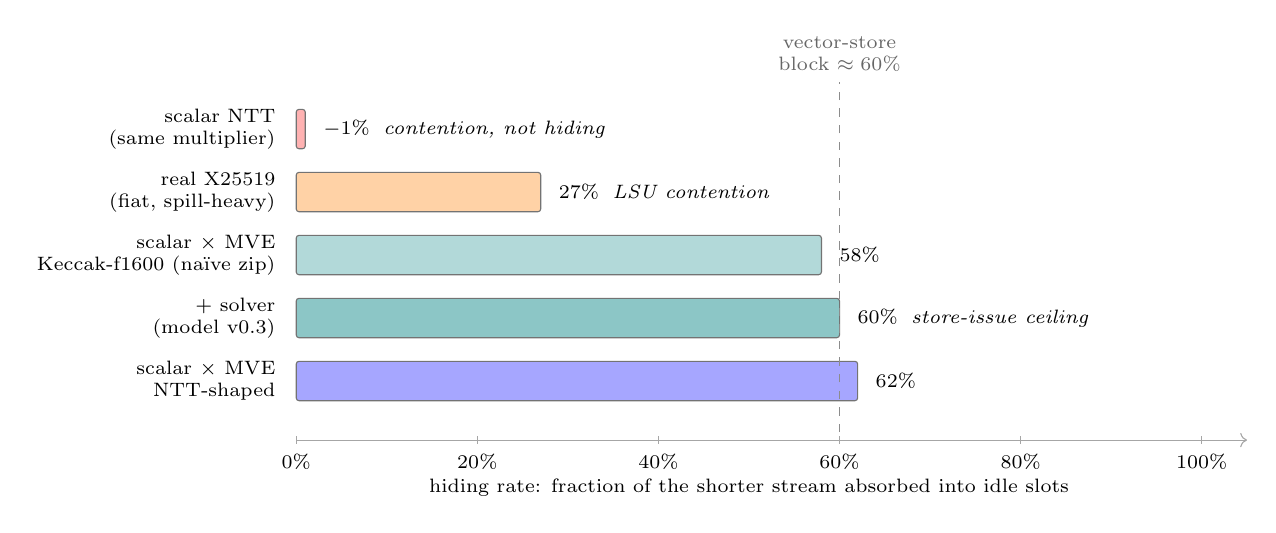
\begin{tikzpicture}[x=0.115cm,y=1cm,font=\small]
  % x: 0--100 (%) → 11.5cm
  \draw[->,gray!70] (0,-0.5) -- (105,-0.5);
  \foreach \p in {0,20,40,60,80,100}
    \draw[gray!70] (\p,-0.45) -- (\p,-0.55) node[below,font=\scriptsize,black] {\p\%};
  \node[below=9pt,font=\scriptsize] at (50,-0.55) {hiding rate: fraction of the shorter stream absorbed into idle slots};
  \tikzset{hb/.style={draw=black!55,rounded corners=1pt,minimum height=0.5cm,
                      inner sep=0pt,anchor=west}}
  % rows: value, y, colour, label, note
  \fill[hb,fill=red!30]    (0,3.2)  rectangle (1,3.7);
  \fill[hb,fill=orange!35] (0,2.4)  rectangle (27,2.9);
  \fill[hb,fill=teal!30]   (0,1.6)  rectangle (58,2.1);
  \fill[hb,fill=teal!45]   (0,0.8)  rectangle (60,1.3);
  \fill[hb,fill=blue!35]   (0,0.0)  rectangle (62,0.5);
  \node[left=4pt,anchor=east,font=\scriptsize,align=right] at (0,3.45) {scalar NTT\\(same multiplier)};
  \node[left=4pt,anchor=east,font=\scriptsize,align=right] at (0,2.65) {real X25519\\(fiat, spill-heavy)};
  \node[left=4pt,anchor=east,font=\scriptsize,align=right] at (0,1.85) {scalar $\times$ MVE\\\keccak{} (na\"ive zip)};
  \node[left=4pt,anchor=east,font=\scriptsize,align=right] at (0,1.05) {\quad$+$ solver\\(model v0.3)};
  \node[left=4pt,anchor=east,font=\scriptsize,align=right] at (0,0.25) {scalar $\times$ MVE\\NTT-shaped};
  \node[right=3pt,anchor=west,font=\scriptsize] at (1,3.45)  {$-1\%$ \;\textit{contention, not hiding}};
  \node[right=3pt,anchor=west,font=\scriptsize] at (27,2.65) {$27\%$ \;\textit{LSU contention}};
  \node[right=3pt,anchor=west,font=\scriptsize] at (58,1.85) {$58\%$};
  \node[right=3pt,anchor=west,font=\scriptsize] at (60,1.05) {$60\%$ \;\textit{store-issue ceiling}};
  \node[right=3pt,anchor=west,font=\scriptsize] at (62,0.25) {$62\%$};
  % ceiling annotation
  \draw[dashed,black!45] (60,-0.4) -- (60,4.05)
     node[above,font=\scriptsize,align=center,black!60] {vector-store\\block $\approx 60\%$};
\end{tikzpicture}
\caption{Hiding rate by pairing and pipe. Two streams that share an execution
resource do not stitch at all (scalar NTT against the UMAAL chain: $-1\%$,
a multiplier tug-of-war); a real, spill-heavy X25519 pairs poorly because its
spill traffic contends with the partner on the load/store unit ($27\%$); moving
the partner to a different pipe (MVE) recovers most of the slot
($58$--$62\%$). The residual is not a scheduling failure but a structural one:
vector stores occupy the scalar issue slot, and $121$ stores $\times\,2$ cycles
account for the exposure exactly (\cref{sec:causes}).}
\label{fig:hiding}
\end{figure}

\section{Plan B Results: Scalar $\times$ MVE, End to End}\label{sec:planb}

Given (a)--(c), the register-file-separated plan is the deployable one: X25519
stays scalar with all 14 GP registers; \keccak{} moves to MVE.

\paragraph{4-way batched MVE \keccak{}.} Armv8.1-M MVE has eight 128-bit
vector registers: exactly four 32-bit-interleaved Keccak states per lane
position. Our generator lays out the permutation with uniformized rotations
across lanes and anchors state addressing so that base-register count shrinks
5$\,\to\,$3$\,\to\,$2 at zero cost (\texttt{vldrw} $\pm$508 offsets). Result:
\textbf{188.5 cycles per state and round vs.\ 229 for pqm4 scalar ($-18$\%)}, with zero
scalar \emph{data} registers---the entire GP file is left to X25519. Lane
transposition glue costs 2.5\% (measured); ML-KEM-768's 43--44 permutations per
operation fill the 4-way queue naturally, and the \xwing{} combiner's single
SHA3-256 permutation rides the same queue as the 45th entry: no extra
mechanism, cost $\leq$ one batch round.

\paragraph{End-to-end at real ratios.} We measure macro-units at the true
operation mix (fiat multiply : batched round = 8:1 for encapsulation, 4:1 for
keygen/decapsulation; real instruction streams, flash-resident at realistic
footprint, correctness-verified) and project by unit counts:

\begin{table}[t]\centering
\caption{\xwing{} operations at real ratios: measured units, projected
operations, and controls.}
\label{tab:final}
\begin{tabular}{lrrr}\toprule
& Serial & Stitched & Saving\\\midrule
Unit 4:1 (keygen/decaps ratio) & 2,008 & 1,772 & $-11.8\%$\\
Unit 8:1 (encaps ratio) & 3,256 & 3,010 & $-7.6\%$\\\midrule
Key generation (projected) & 544k & 482k & \textbf{11.4\%}\\
Encapsulation (projected) & 886k & 821k & \textbf{7.3\%}\\
Decapsulation (projected) & \multicolumn{2}{c}{(4:1, as keygen)} & \textbf{$\sim$11.4\%}\\\midrule
Control: coarse alternation (3:3 unit) & 3,220 & 3,199 & $-0.7\% \approx 0$\\
Same unit, instruction-level stitch & 3,220 & 2,943 & $-8.6\%$\\\bottomrule
\end{tabular}\end{table}

Two control results matter. Coarse alternation---switching algorithms at
function granularity, the ``easy'' software answer---recovers nothing
($-0.7\%$): the gain genuinely lives at instruction granularity. And the
balance law is visible: 4:1 units save more than 8:1 (11.8\% vs.\ 7.6\%),
because saving is bounded by the hideable stream B share; the 1:1 unit sits at
8.1\% (partially hidden).

\paragraph{Verdict against the pre-registered bar.} We had committed to a 20\%
end-to-end bar for the aggressive narrative. 7--11\% misses it. Per the
pre-registered fallback, this paper reports the automation, the decomposition,
and the MVE kernel as the contributions, and the thin-but-real end-to-end win
as the measured answer to the Stage-4 question (``does the gain survive whole
operations?''---yes, at 7--11\%).

\section{Constant Time}\label{sec:ct}

Stitching adds no timing channel, by construction and by measurement.
\emph{Structurally}: the transform is compile-time only---it reorders
instructions, renames registers, and (via \texttt{-ffixed} compilation) inserts
spills to fixed stack/DTCM offsets; it inserts zero branches and no
secret-dependent addressing. Both input streams are constant-time to begin with
(fiat-crypto's generation guarantee; Lenngren's masked cswap ladder; Keccak is
a fixed permutation; the 4-way queue length is the per-operation constant
43--45). On M85, integer and MVE latencies are operand-independent and
ITCM/DTCM are 0-wait, so a fixed instruction sequence implies fixed cycles.
\emph{Empirically}: the stitched fiat$\times$MVE kernel measured on two
unrelated input sets gives median $\Delta = 0$ cycles (979,065 vs.\ 979,065 at
$\times$1000 loop resolution), and Unicorn instruction counts agree on two
inputs for every kernel. We did not run dudect-style statistics: with no
physical path for value-dependent timing in this configuration, the two-input
check is confirmation, not evidence of first resort. Power side channels are
out of scope.

\section{Related Work}\label{sec:related}

Intel's stitching \cite{Intel10} is the origin; it is hand-placed, unmeasured
on the waste side, symmetric-only, and out-of-order-x86-only.
\slothy{} \cite{Slothy22,SlothyM7_25} superoptimizes single streams; our
extension makes the two-stream problem---including inter-stream register
reallocation, which no fixed-partition manual technique can express---a solver
problem. Becker--Kannwischer's scalar/vector Keccak \cite{BK22} pioneered
mixed-register-file execution on Cortex-A; our pairing-spectrum experiment
quantifies exactly when that works on in-order M-class (loads pair, stores
block). Multi-core hybrid parallelization \cite{DualCore25,ParHyb26} is
orthogonal: it buys overlap with silicon, we recover it from issue slots.
Hybrid cost accounting on M4 \cite{Sim26} anchors our baselines and supplied the
stream-balance estimate we pre-registered; the M85 measurement confirms its
direction, with X25519 the longer stream and coverage dilution---not slot
capacity---setting the bound. ML-KEM implementation baselines: pqm4 \cite{pqm4},
FIPS~203 \cite{FIPS203}.

\section{Conclusion}\label{sec:conclusion}

On an in-order dual-issue core, function stitching of X25519 and Keccak is
real, automatable, and thin: 7--11\% end to end against a 21--27\% bound, with
every point of the gap accounted for by an isolating experiment. The honest
summary for practitioners: (i) if you can spend a vector unit, spend it on
batching (our 4-way MVE Keccak is 18\% faster per state before any stitching)
and take stitching's 7--11\% on top where the ratio is favorable; (ii) do not
hand-schedule---model accuracy decides wins (a single mis-priced latency
flipped our solver from losing by 30\% to winning), and the extended solver
plus the C-\texttt{-ffixed}-solve pipeline is reusable; (iii) on cores without
reorder hardware, the pairing table (which instruction classes co-issue) is the
design document. The tools, harness, kernels, KATs, and pre-registration
documents ship as artifacts.

\paragraph{Limitations.} Macro-unit fidelity (ladder control flow and
absorb/squeeze glue, bounded at 2.5\%, sit outside the measured units); single
platform (Cortex-M55 untested---\todo{M55 board}); the scalar dual-issue model
remains TRM-unvalidated in its pairing details beyond the rules measured here.

Energy is deliberately out of scope. This is a scheduling study on a
fixed-clock in-order core: every claim we make is a cycle count, and the
quantity we optimise---issue slots recovered by interleaving two instruction
streams---maps to energy only through the same clock. We therefore report
cycles throughout and make no joule-per-operation claim. The one place where
this could hide something is the MVE path of Plan~B, since vector units carry
a different power profile than the scalar pipeline they displace; a scalar
vs.\ vector energy comparison at equal cycle count is future work requiring
power instrumentation, and would refine---but not overturn---the slot-recovery
accounting presented here.

\printbibliography

\appendix
\section{Measurement Details}
EK-RA8M1, 480\,MHz, FSP BSP clocks; code ITCM, data DTCM; DWT \texttt{CYCCNT}
medians of $N{=}100$, 25-cycle calibration; Unicorn instruction counts (IT
blocks counted individually; may differ from \texttt{INST\_RETIRED} by a few
percent). PMU event counters were nonfunctional on our board specimen;
cycle+emulated-count arithmetic replaces front/back-end stall attribution.
Version pins: pqm4 \texttt{cc2c1b992b60}, upstream \slothy{}
\texttt{241093fa5ddc} (+ our patch v0.1--v0.4), Lenngren X25519 vendored with
license. The harness auto-verifies every kernel (KAT/reference match) before
timing; a constant-time PASS/FAIL line accompanies each harvest.

\section{Reproduction Hazards}
Loop bodies need \texttt{.balign 16} ($\pm$1 cycle/iteration otherwise); large
ITCM functions must use \texttt{movw}/\texttt{movt} instead of literal pools;
DTCM stack switches must also move \texttt{MSPLIM}; \texttt{CYCCNT} writes are
ignored while the PMU is disabled; the vendor IDE may silently shrink the
TrustZone flash partition below the firmware size (fix via the partition CLI).
Doubleword accesses must be split and spill slots never reused when feeding
compiler output to the solver (\cref{sec:auto}).

\end{document}
